%%%%%latex preamble%%%%%
\documentclass[titlepage]{article}\usepackage[]{graphicx}\usepackage[]{color}
%% maxwidth is the original width if it is less than linewidth
%% otherwise use linewidth (to make sure the graphics do not exceed the margin)
\makeatletter
\def\maxwidth{ %
  \ifdim\Gin@nat@width>\linewidth
  \linewidth
  \else
  \Gin@nat@width
  \fi
}
\makeatother


\usepackage{listings}
\definecolor{mygreen}{rgb}{0,0.6,0}
\definecolor{mygray}{rgb}{0.5,0.5,0.5}
\definecolor{mymauve}{rgb}{0.58,0,0.82}
\lstset{ %
  backgroundcolor=\color{white},   % choose the background color; you must add \usepackage{color} or \usepackage{xcolor}
  basicstyle=\footnotesize,        % the size of the fonts that are used for the code
  breakatwhitespace=false,         % sets if automatic breaks should only happen at whitespace
  breaklines=true,                 % sets automatic line breaking
  captionpos=b,                    % sets the caption-position to bottom
  commentstyle=\color{mygreen},    % comment style
  deletekeywords={...},            % if you want to delete keywords from the given language
  escapeinside={\%*}{*)},          % if you want to add LaTeX within your code
  extendedchars=true,              % lets you use non-ASCII characters; for 8-bits encodings only, does not work with UTF-8
  frame=single,                    % adds a frame around the code
  keepspaces=true,                 % keeps spaces in text, useful for keeping indentation of code (possibly needs columns=flexible)
  keywordstyle=\color{blue},       % keyword style
  language=Python,                 % the language of the code
  morekeywords={*,...},            % if you want to add more keywords to the set
  numbers=left,                    % where to put the line-numbers; possible values are (none, left, right)
  numbersep=5pt,                   % how far the line-numbers are from the code
  numberstyle=\tiny\color{mygray}, % the style that is used for the line-numbers
  rulecolor=\color{black},         % if not set, the frame-color may be changed on line-breaks within not-black text (e.g. comments (green here))
  showspaces=false,                % show spaces everywhere adding particular underscores; it overrides 'showstringspaces'
  showstringspaces=false,          % underline spaces within strings only
  showtabs=false,                  % show tabs within strings adding particular underscores
  stepnumber=2,                    % the step between two line-numbers. If it's 1, each line will be numbered
  stringstyle=\color{mymauve},     % string literal style
  tabsize=2,                       % sets default tabsize to 2 spaces
  title=\lstname                   % show the filename of files included with \lstinputlisting; also try caption instead of title
}
\usepackage{alltt}
\usepackage[sc]{mathpazo}
\usepackage{amsmath, amsthm, amssymb}
\usepackage{graphicx}
\usepackage[T1]{fontenc}
\usepackage{geometry}
\geometry{verbose,tmargin=2.5cm,bmargin=2.5cm,lmargin=1.5cm,rmargin=1.5cm}
\setcounter{secnumdepth}{2}
\setcounter{tocdepth}{2}
\usepackage{url}
\usepackage[unicode=true,pdfusetitle,
  bookmarks=true,bookmarksnumbered=true,bookmarksopen=true,bookmarksopenlevel=2,
breaklinks=false,pdfborder={0 0 1},backref=false,colorlinks=false, hidelinks]
{hyperref}
\hypersetup{pdfstartview={XYZ null null 1}}
\usepackage{float}
\usepackage{bm}
\usepackage{tikz}
 %changes default sectioning commands -> 1,a, etc.
%\usepackage{breakurl}
\renewcommand{\thesubsection}{(\alph{subsection})}
\renewcommand{\thesubsubsection}{\roman{subsection}.}
\usepackage{lastpage}
\usepackage{fancyhdr}
\pagestyle{fancy}
\usepackage{tikz-qtree}

%%% Header and Footer %%% 
\lhead{}
\chead{\leftmark}
\rhead{}
\lfoot{Aaron Gonzales; Algorithms}
\cfoot{Homework 7}
\rfoot{Page \thepage\ of \pageref{LastPage}}
\IfFileExists{upquote.sty}{\usepackage{upquote}}{}

\begin{document}

\title{Homework 7, CS561, Fall 2014}
\author{Aaron Gonzales}
\maketitle


%%%% useful align for this
\section{26.2 - 4: Min cut/Max flow}
  \begin{quote}
    \textbf{In the example of Figure 26.6, what is the minimum cut corresponding
    to the maximum flow shown? Of the augmenting paths appearing in the
    example, which one cancels flow?}
  \end{quote}

  \begin{figure}
    \begin{center}
    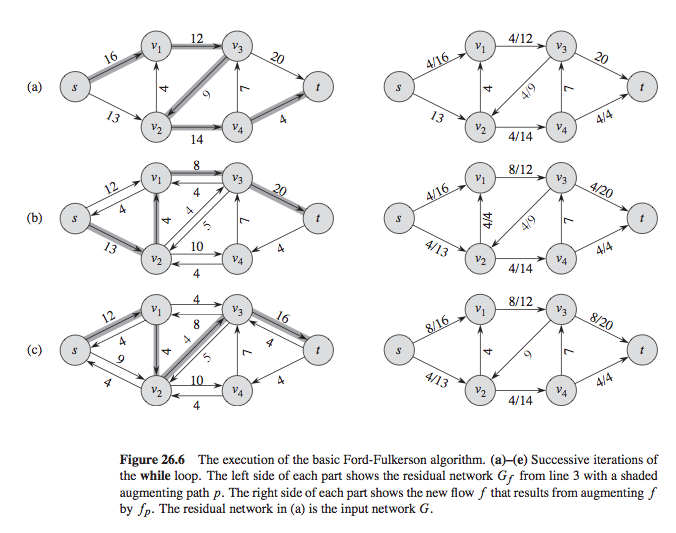
\includegraphics[scale=0.40]{26.6a.png}\\*
    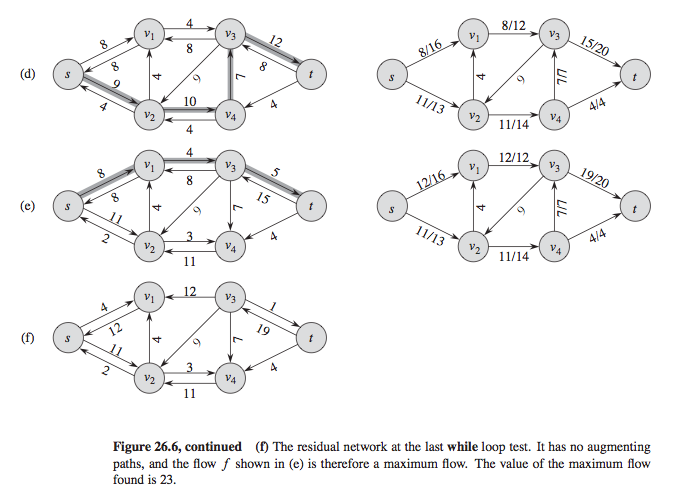
\includegraphics[scale=0.40]{26.6b.png}\\*
  \end{center}
  \label{fig:26.6a}
  \caption{Figure 26.6 a-f from CLRS 3rd edition pdf}
  \end{figure}
  \subsubsection{Answer:}
  Our cut will partition the graph into two sets:
  \[ \{s, v_1, v_2, v_4\}, \{v_3, t\} \]
  which respect the total augmenting flow in 26.6(c) of 23.


\section{26.2 - 11 : connectivity}
  \begin{quote}
    \textbf{The edge connectivity of an undirected graph is the minimum number
      $k$ of edges that must be removed to disconnect the graph. For example,
      the edge connectivity of a tree is 1, and the edge connectivity of a
      cyclic chain of vertices is 2. Show how to determine the edge
      connectivity of an undirected graph $G = (V,E) $ by running a
      maximum-flow algorithm on at most $|V|$ flow networks, each having $O(V)$
      vertices and $O(E)$ edges.}
  \end{quote}

  \subsubsection{Answer:}
  As a reminder, a min cut can be stated as finding a subset $S \in V$ of a graph $G =
  (V,E)$such that $S \neq 0$ with edges $C$ crossing from $A$ to $V-A$ minimized.
  For this problem, the cost of the cut can be the number of edges $||C||$ that
  cross the cut. Here, we want to find the min cut of some cost equal to $k$.
  Removing the edge set  $C$ from the graph clearly disconnects the graph. 

  Our algorithm can be described as follows:
  Let $s$ be some vertex in $V$ chosen at random. give a weight of 1 to every
  edge in the graph. For every other vertex $t_i$ in $G$, find the min cut from $s$
  to $t_i$ and save the number of edges that cross the min cut. Upon
  completion, return minimum number $k$ from the process and you have the
  edge connectivity value of the graph. The algorithm examines $\Theta(V-1) =
  \Theta(V)$ nodes and using Ford-Fulkerson gives us a total runnig time of
    $O(E\times V^2)$.

  Note that Karger's algorithm can answer this question as well in a
  randomized way of contracting edges in a graph by merging nodes together
  into a series of multigraphs until two nodes remain that represent a cut in
  the original graph. It can run with total time $O(V^2\, log\, V)$
  depending on implementation and would work far more quickly than the above
  answer\footnote{\url{http://en.wikipedia.org/wiki/Karger\%27s_algorithm}}. 


\section{Perfect Matchings}
  \begin{quote}
      \textbf{A bipartite graph is a graph that contains no cycle with an odd
      number of edges. Recall from the wrestler problem that a graph, $G = (V,
      E)$ is
    bipartite iff $V$ can be partitioned into two sets $L, R$ such that all
    edges in $E$
    have one endpoint in $L$ and one endpoint in $R$. A matching in a graph is a set of
    edges $E' \in E$ such that each vertex in $V$ is matched at most once, i.e. it is
    incident to a most one edge in $E'$. A perfect matching is a matching where every
    vertex is matched, i.e. is incident to exactly one edge in $E'$. For a set of
    vertices $S \in V$, let $N(S)$ be the set of all neighbors of $S$, i.e. $\{y
    \in V : (x,y) \in \, E $ for some $x \in S\}$ \\*
    Assume we are given a bipartite graph where $|L| = |R|$. Prove that there is a
    perfect matching in $G$ iff $|N(S)| \geq |S|$ for all $S \in L$.
    Hint: Use the Max flow/Min Cut Theorem}
  \end{quote}
  \subsubsection{Answer:}
    If we let assign unit (1) weight to each edge in the graph and add a source
    vertex $s$ that is connected from itself to each vertex in $L$ and a sink vertex $t$
    that takes a directed edge from each vertex in $R$, we can model this as a
    network flow problem. (In other words, direct all the edges from the source
    on the left to the sink of the right). Let this restructured graph be
    called $G'$. 
  \begin{proof}
    Given that our graph has $|L| = |R|$, let $n = |L|$. 
    Suppose for sake of contridiction that $G$ contains no perfect matching. If
    this is true, then the size of the maximum match in $G$ is at most $\leq n
    -1$ and as such the max flow in $G'$ is $\leq n-1$. As such, $G'$ must have
    a cut $C$ with at least capacity $n-1$. 

    Let $L_a$ be the left vertices in cut $C$, $L_b$ be the remaining vertices
    in $L$. Let $R_a$ and $R_b$ be defined the same for the right side. The
    flow capacity of the edges crossing $C$ is the same as the number of edges
    crossing $C$, which is $|L_b| + |R_a| + |L_a,R_b|$. 
    We now have 
    \[n-1 \geq |L_b| + |R_a| + |L_1, R_2|\]
    and this reduces to 
    \[ |N(L_a) \leq |R_a| + |L_a,R_2| \] because our $L_a$ neighboorhood can
    only have edges from $L_a, R_b$ in $R_2$. 
    \[ L_a \leq N(L_a) + 1 \] and we conclude the proof.
  \end{proof}

  



\section{Image segmentation}
  \begin{quote}
    \textbf{Consider the following problem related to segmenting the pixels
      of an image between foreground and background. We have a picture that
      consists of $n$ pixels. We represent this as an undirected graph $G =
      (V,E)$ where $V$ is the set of pixels and there is an edge $(i,j) \in
      E$ iff pixel $i$ and pixel $j$ are neighbors in the image
      \footnote{Note that we'd commonly expect this graph to be a grid, but
        in fact we want to handle any arbitrary graph (to handle, e.g., 3-D
        images, wrapped and warped images, etc)}}. \\* 
        \textbf{We want to find
        a good segmentation, which is an assignment of each pixel to either
        the foreground or the background.  For each pixel $i$, we have a
        likelihood $a_i$ that $i$ belongs to the foreground and a likelihood
        $b_i$ that $i$ belongs to the background. These likelihood values are
        all non-negative. Additionally, for each edge $(i, j) \in E$, we have
        a non-negative separation penalty $p_i,j$ which is charged if one of
        $i$ or $j$ is assigned to the foreground and the other is assigned to
        the background.  Our problem then is to find a partition of the set
        of pixels into sets $A$ and $B$ so as to maximize:}
        \begin{align}
        \label{imgseg_max}
        L(A, B) = \sum_{i \in A}  a_i + \sum_{i \in B} b_i − \sum_{(i,j) \in E,
          | A \cap \{i,j\} | = 1} p_{i,j} 
        \end{align}
      \textbf{Give an efficient algorithm to solve this problem}
  \end{quote}

  \subsubsection{Answer:}

  This maximization problem stated in \ref{imgseg_max} can be formulated as a
  minimization problem instead, that is,
  \begin{align}
    \label{imgseq_min}
    \max(a) = \sum_{i \in A}  a_i + \sum_{i \in B} b_i − \sum_{(i,j) \in E, | A \cap \{i,j\} | = 1} p_{i,j} 
  \end{align}
is equivalent to
  \begin{align}
    \label{blah}
    \min (g') = \sum_{i \in B} f_i + \sum_{i \in A} b_i + \sum_{i \in P| j \in Q j \in P|i \in Q } p_{ij}. 
  \end{align}

The above minimization problem can be formulated as a minimum-cut problem by
constructing a network where the source is connected to all the pixels with
capacity $a_i$ and the sink is connected by all the pixels with capacity $b_i$
Two directed edges $i,j$ and $j,i$ with $p_{ij}$ capacity are added between two adjacent
pixels. The s-t cut-set then represents the pixels assigned to the foreground
in $A$ and pixels assigned to background in $B$ as we have minimized our
desired quantity from equation \ref{blah}.



\section{Exercise 29.2-2 (Linear Program)}
  \begin{quote}
    \textbf{Write out explicitly the linear program corresponding to finding
    the shortest path from node $s$ to node $y$ in Figure 24.2(a).}
  \end{quote}
\usetikzlibrary{arrows}
\begin{figure}
  \begin{center}
	\begin{tikzpicture}[->,>=stealth',shorten >=1pt,auto,node distance=3cm,
	  thick,main node/.style={circle,fill=blue!20,draw,font=\sffamily\Large\bfseries}]

	  \node[main node] (1) {3};
	  \node[main node] (2) [right of=1] {9};
	  \node[main node] (3) [below of=2] {11};
	  \node[main node] (4) [below of=1] {5};
	  \node[main node] (5) [below left of=1] {0};

	  \path[every node/.style={font=\sffamily\small}]
		(1) edge node [above] {6} (2)
			 edge [bend right] node[left] {2} (4)
			%edge [loop above] node {0.1} (1)
		(2) edge[bend right] node [bend right] {2} (3)
			%edge [loop left] node {0.4} (2)
			%edge [bend right] node[left] {0.1} (3)
		(3) edge [bend right] node [right] {7} (2)
                    edge node [below right] {3} (5)
		(4) edge [bend right] node [above left] {1} (1)
                        edge node[below] {6} (3)
                        edge node {4} (2)
		(5) edge node [above left] {3} (1)
                    edge node [below left] {5} (4);
                    %edge node [left] {5} (2);
			%edge [loop right] node {0.6} (4)
	\end{tikzpicture}
  \end{center}
\caption{Figure 24.2 from CLRS}
\label{fig:figure1}
\end{figure}
  \subsubsection{Answer:}
  We have several constraints for our linear program. Let $d_a$ be the
  distance up to a node $a$. Our constraints follow:
  \begin{align*}
    d_s = & 0 \\
    d_t \leq & d_s + 3 \\
    d_t \leq & d_y + 1 \\
    d_y \leq & d_s + 5 \\
    d_y \leq & d_t + 2 \\
    d_x \leq & d_t + 6 \\
    d_x \leq & d_z + 7 \\
    d_z \leq & d_y + 6 \\
    d_z \leq & d_x + 2 
  \end{align*}
\section{Exercise 29.2-4 (Network Flow as an LP)}
  \begin{quote}
    \textbf{Write out explicitly the linear program corresponding to finding
      the maximum flow in Figure 26.1(a) (Figure \ref{fig:26a} on page
      \pageref{fig:26a}.}
  \end{quote}
  \begin{figure}
    \begin{center}
    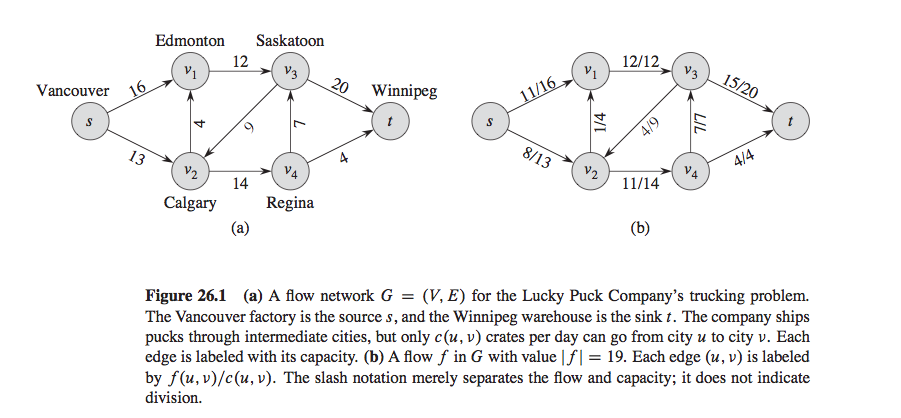
\includegraphics[scale=0.40]{26.1a.png}\\*
    \end{center}
    \caption{Figure 26.1a from CLRS 3rd edition PDF}
    \label{fig:26a}
  \end{figure}
  \subsubsection{Answer:}
  Note that a network flow problem would have the following global constraints:
  Conservation of Flow
  \begin{align}
    \sum_{\text{outflow}} x_j - \sum_{\text{inflow}}x_j = 0
  \end{align}
  Our program would have the following constraints:
  Let $f{i \to j} $ be a path from node $i$ to node $j$. Note that we must
  preserve conservation of flow and that our program will have constraints
  respecting flow and capacity of edges.

  \begin{equation}
    \begin{aligned}
      f_{s \to s} &= 0 \\
      f_{s \to v_1} &\leq 16  \\
      f_{s \to v_2} &\leq 13   \\
      f_{v_1 \to v_3} &\leq 12  \\
      f_{v_2 \to v_1} &\leq 4  \\
      f_{v_2 \to v_4} &\leq 14  \\
      f_{v_3 \to v_2} &\leq 9  \\
      f_{v_3 \to t} &\leq 20  \\
      f_{v_4 \to v_3} &\leq  7 \\
      f_{v_4 \to t} &\leq  4 
    \end{aligned}
  \end{equation}

  we also have the following constraints on capacity:
  \begin{equation}
    \begin{aligned}
      f_{s \to v_1} + f_{v_2 \to v_1} &=  f_{v_1 \to v_3} \\
      f_{s \to s} + f_{s \to s} &=  f_{s \to s} \\
      f_{s \to s} + f_{s \to s} &=  f_{s \to s} \\
      f_{s \to s} + f_{s \to s} &=  f_{s \to s} \\
      f_{s \to s} + f_{s \to s} &=  f_{s \to s} \\
      f_{s \to s} + f_{s \to s} &=  f_{s \to s} \\
      f_{s \to s} + f_{s \to s} &=  f_{s \to s} \\
      f_{s \to s} + f_{s \to s} &=  f_{s \to s} \\
      f_{s \to s} + f_{s \to s} &=  f_{s \to s}
    \end{aligned}
  \end{equation}

\section{Rock, Paper, Scissors}
  \begin{quote}
    \textbf{Rock, Paper, Scissors is a simple 2 person game. In a given round,
    both players simultaneously choose either Rock, Paper or Scissors. If they
    both choose the same object, it’s a tie. Otherwise, Rock beats Scissors;
    Scissors beats Paper; and Paper beats Rock. Imagine you’re playing the
    following betting variant of this game with a friend. When Scissors beats
    Paper, or Paper beats Rock, the loser gives the winner \$1. However, in the case
    when Rock beats Scissors, this is called a \textbf{smash}, and the loser must give the
    winner \$10.}
  \end{quote}

  \subsection{Say you know that your friend will choose Rock, Scissors or
        Paper, each with probability $\frac{1}{3}$. Write a linear program to
        calculate the probabilities you should use of choosing each object in
        order to maximize your expected winnings. Let $p_1,p_2,p_3$ be variables
        associated with the best way of choosing Rock, Scissors and Paper
        respectively. Note: If you want to check your work, there are several free
        linear program solvers on the Internets: check the Wikipedia page on linear
        programming.} 
  \subsubsection{Answer:}

  Let $\rho = \{p_{r}, p_{s}, p_{p}\}$ be the set of variables associated with us choosing Rock,
 Scissors and Paper respectively. Maximize: 
  if $p_1, p_2, p_3$ are the probabilities of choosing the 
  \begin{align}
    \label{rps:a}
    & \frac{1}{3}\left(10*p_{r} - 1*p_{s} - 10*p_{s} + 1*p_{s} +  1*p_{p} - 1*p_{p}\right) \\ 
    & \text{ with the following constraints:} \\ 
       & 0 \leq p_r, p_s, p_p \leq 1 \\ 
       & \sum \rho = 1  \text{  (abuse of notation, sorry)}
  \end{align}



  \subsection{Now say that your friend is smart and, also,
        clairvoyant: she will magically know the exact probabilities you are
        using and will respond optimally. Write another linear program to
        calculate the probabilities you should now use in order to maximize your
        expected winnings. \\* Hint 1: If your opponent knows your strategy, her
        strategy will be to choose one of the three objects with probability 1.
      \\* Hint 2: Review the LP you wrote for the shortest paths problem.}
  \subsubsection{Answer:}
  Let $P = $ our profit and $Q = $ our friend's profit. Let $\rho = \{P_r, P_p, P_s\}$ be
  our probabilities of choosing rock, paper, or scissors. Let $Q_r, Q_p, Q_s$
  be our friend's winnings when she chooses rock, paper, or scissors,
  respectively.
  Then let her winnings be defined as
  \begin{equation}
    \begin{aligned}
      Q_r =& P_p - 10P_s &\text{she picks rock} \\
      Q_p =& P_s - P_r   &\text{she picks paper} \\
      Q_s =& 10P_r - P_p &\text{she picks scissors} \\
    \end{aligned}
    \label{rps:winnings}
  \end{equation}
  Then we want to maximize her winnings in \ref{rps:winnings} in such a way to
  minimize our winnings. 

  \begin{equation}
    \begin{aligned}
      \label{rps:constraints}
      \max(Q) =& \\
      &\min \begin{cases} Q_r =& P_p - 10P_s \\
                    Q_p =& P_s - P_r   \\
                    Q_s =& 10P_r - P_p \\
                  \end{cases} \\
       0 \leq p_1, p_2, p_3 &\leq 1 \\ 
       \sum \rho  &= 1  \text{  (abuse of notation, sorry)}
    \end{aligned}
  \end{equation}

  
  \vspace{3cm}

\section{Independent-Set}
  \begin{quote}
  \textbf{The problem INDEPENDENT-SET asks: Does there exist a set of $k$
  vertices in a graph $G$ with no edges between them? Show that this problem is
  NP-Complete. (hint: Reduce from CLIQUE)}
  \end{quote}
  \subsubsection{Answer:}
  \begin{proof} Via reduction from CLIQUE
    \subsubsection{Part one:NP}
    INDEPENDENT-SET is in NP. Given a vertex set $S$ returned from the
    algorithm we can indeed check that $S$ is an independent set of vertices
    by checking that each vertex in $S$ is in the graph and that there are no
    edges between any two vertices in $S$. A simple BFS or DFS will handle this
    in $O(V+E)$ time and INDEPENDENT-SET $\in $ NP.
    \subsubsection{Part two: NP-Hard}
    INDEPENDENT-SET is NP-Hard. Recall that an instance of CLIQUE is a graph
    $G$ and an integer $k$. We can convert an instance of CLIQUE to
    INDEPENDENT-SET as such: Let $G_c$ be the complement graph of $G$ and pass
    $G_c,k$ to INDEPENDENT-SET.
    Assume that there is a clique $C$ of size $k \in G$. For any $u,v \in C,
    (u,v) \in E$. Thus, $(u,v) \notin E_c$ and the vertices of $C$ form an
    independent set in $G_c$ and $G_c$ is a yes instance from INDEPENDENT-SET.
    If $G_c$ is a yes isntance from INDEPENDENT-SET, then any $u,v \in I,
    (u,v,) \notin E_c$ and $u,v \in E$ and the vertices in I form a clique in
    G. 


    INDEPENDENT-SET is both NP and NP-HARD and as such IS $\in$ NP-Complete.
  \end{proof}








\section{Exercise 34.5-1 (Subgraph Isomorphism)}
  \begin{quote}
    \textbf{The subgraph-isomorphism problem takes two undirected graphs $G_1$ and
    $G_2$, and it asks whether $G_1$ is isomorphic to a subgraph of $G_2$. Show that the
    subgraph-isomorphism problem is NP-complete.}
  \end{quote}
  \subsubsection{Answer:}
  In order to show NP-completeness, we must state the problem as a decision
  problem. We can ask if a given graph is isomorphic to a subgraph of another
  graph, and in this case, if $G_1$ is isomorphic to a subgraph of $G_2$, the
  answer is ``true'' and ``false'' otherwise. 
  Let it be stated that to be isomorphic to another graph, a graph $G = (V,E)$
  must have a subgraph $G_0 = (V_0, E_0) : V_0 \subseteq V, E_0 =
  E\cap(V_0\times V_0)$ such that $G_0 \cong H$? Does a mapping $f: V_0 \to V'$
  exist such that vertices $v_1, v_2 \in E_0 \Leftrightarrow (f(v_1), f(v_2))
  \in E'$?
  \begin{proof}
    \subsubsection{SI is in NP}
    there can be $O(n^2)$ pairs in the list of nodes comprising $G_1$ and the
    subgraph of $G_2$ that we must check to verify that it is isomorphic. This
    polynomial time check verifies that SI is in NP.
    \subsubsection{SI is NP-Complete}
    By reduction from CLIQUE. \\
    CLIQUE $\leq_P$ SUBGRAPH ISOMORPHISM. Let $(G = (V,E)k)$ be an input for
    CLIQUE and let $G_1$ to be the complete graph on $k$ vertices and $G_2$ to
    be the graph $G$. $G_1,G_2 \in$ SUBGRAPH ISOMORPHISM iff $G,k \in CLIQUE$.
    If $G$ has a $k$-clique, then $G$ has the $k$-graph as a subgraph and
    $G,G_k$ is a yes instance of the problem. As this is at least as hard as
    Clique, we conclude that SUBGRAPH-ISOMORPHISM is NP-Hard $\implies$ NP-Complete.
  \end{proof}



\end{document}
